% Marius-Juston 2026
\documentclass[tikz,border=0pt]{standalone}
\usepackage{amsmath}
\usetikzlibrary{arrows.meta, decorations.markings, calc}

\begin{document}
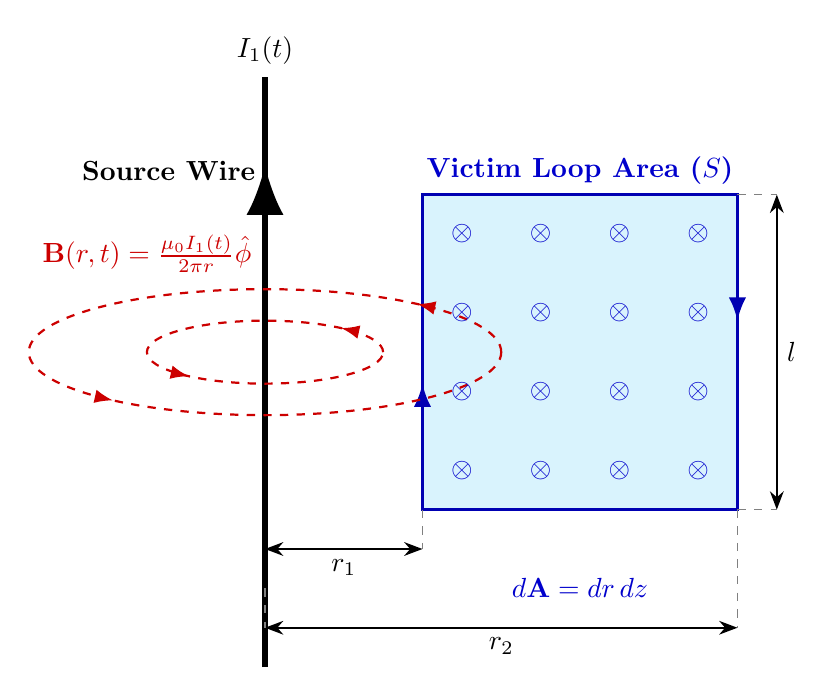
\begin{tikzpicture}

    % Source Wire definition with current directional arrow
    \draw[line width=2pt, postaction={decorate,decoration={markings, mark=at position 0.85 with {\arrow{Latex[scale=1.5]}}}}] 
        (0,-1) -- (0,6.5) node[above] {$I_1(t)$};
    \node[left, font=\bfseries] at (0,5.3) {Source Wire};
    
    % Victim Loop geometry definition
    \draw[line width=1.2pt, fill=cyan!15, draw=blue!70!black,    decoration={
        markings,
        mark=at position 0.1 with {\arrow{Latex}},
        mark=at position 0.6 with {\arrow{Latex}}
      },
      postaction={decorate}] (2,1) rectangle (6,5);
    \node[blue!80!black, font=\bfseries] at (4, 5.3) {Victim Loop Area ($S$)};
    
    % Boundary distances (r1, r2, l)
    \draw[<->, >=Stealth, thick] (0,0.5) -- (2,0.5) node[midway, below] {$r_1$};
    \draw[<->, >=Stealth, thick] (0,-0.5) -- (6,-0.5) node[midway, below] {$r_2$};
    \draw[<->, >=Stealth, thick] (6.5,1) -- (6.5,5) node[midway, right] {$l$};
    
    % Extension lines for dimensional clarity
    \draw[dashed, gray] (2,1) -- (2,0.5);
    \draw[dashed, gray] (6,1) -- (6,-0.5);
    \draw[dashed, gray] (0,0) -- (0,-0.5);
    \draw[dashed, gray] (6,5) -- (6.5,5);
    \draw[dashed, gray] (6,1) -- (6.5,1);
    
    % Magnetic Field (B) representation
    % Amperian contours
    \draw[thick, red!80!black, dashed,    decoration={
        markings,
        mark=at position 0.1 with {\arrow{Latex}},
        mark=at position 0.6 with {\arrow{Latex}}
      },
      postaction={decorate}] (0,3) ellipse (1.5 and 0.4);
    \draw[thick, red!80!black, dashed,    decoration={
        markings,
        mark=at position 0.1 with {\arrow{Latex}},
        mark=at position 0.6 with {\arrow{Latex}}
      },
      postaction={decorate}] (0,3) ellipse (3 and 0.8);
    
    % Vector field penetrating the surface (into the page)
    \foreach \x in {2.5, 3.5, 4.5, 5.5} {
        \foreach \y in {1.5, 2.5, 3.5, 4.5} {
            \node[blue!80!black] at (\x,\y) {$\otimes$};
        }
    }
    
    % Field equation annotation
    \node[red!80!black] at (-1.5, 4.25) {$\mathbf{B}(r,t) = \frac{\mu_0 I_1(t)}{2\pi r} \hat{\phi}$};
    \node[blue!80!black] at (4, 0) {$d\mathbf{A} = dr \, dz$};

\end{tikzpicture}
\end{document}